\documentclass{article}
\usepackage[utf8]{inputenc}
\usepackage[francais]{babel}
\usepackage[T1]{fontenc}
\usepackage{graphicx}    
\usepackage{eurosym}
\usepackage{verbatim}      
\usepackage{amsmath, amsthm}                             
\usepackage{latexsym}           
\usepackage{gensymb}

\usepackage{amssymb}
\usepackage{tabularx}
\usepackage{setspace}
\usepackage{listings}
\usepackage{geometry}
\usepackage{fancyhdr}
\usepackage{enumitem}
\usepackage{colortbl}
\usepackage[dvipsnames]{xcolor}
\usepackage{booktabs} 
\usepackage{moreverb}
\usepackage{mathtools}
\usepackage{pdfpages}

\usepackage{cancel,soul,ulem}

\DeclareMathAlphabet{\mathonebb}{U}{bbold}{m}{n}
\newcommand{\one}{\ensuremath{\mathonebb{1}}}

\usepackage{color}
\usepackage{multirow}
%\usepackage{float}
\definecolor{gris25}{gray}{0.75}
\usepackage{colortbl}
\usepackage{fancyhdr}
\usepackage{amsmath,amsfonts,amssymb}
\usepackage{titlesec}
\usepackage{supertabular}
\usepackage{longtable}

\usepackage{caption}
\usepackage{subcaption}


\usepackage{listings}
\definecolor{dkgreen}{rgb}{0,0.4,0}
\definecolor{gray}{rgb}{0.5,0.5,0.5}
\definecolor{mauve}{rgb}{0.58,0,0.82}

\usepackage{algorithm2e}
\newcommand{\algorithmicrequire}{\textbf{Input:}}
\newcommand{\algorithmicensure}{\textbf{Output:}}
\newcommand{\sign}{\text{sign}}
\newcommand{\argmin}{\text{argmin}}
\newcommand{\Cut}{\text{Cut}}
\newcommand{\Vol}{\text{Vol}}
\newcommand{\RCut}{\text{RCut}}
\newcommand{\NCut}{\text{NCut}}
\newcommand{\NCC}{\text{NCC}}
\newcommand{\RCC}{\text{RCC}}
\newcommand{\PR}{\text{Pr}}

\usepackage{blkarray}

\usepackage{lipsum}

\newcommand{\exedout}{%
  \rule{0.8\textwidth}{0.5\textwidth}%
}

\newcommand{\tw}[1]{\textcolor{red}{\bf [TW:~#1]}}

\definecolor{dkyellow}{cmyk}{0, 0, 0.2, 0}
\lstset{
  language=R,                % the language of the code
  basicstyle= \footnotesize,      % the size of the fonts that are used for the code
  numbers=left,                   % where to put the line-numbers
  numberstyle=\tiny\color{gray},  % the style that is used for the line-numbers
  stepnumber=2,                   % the step between two line-numbers. If it's 1, each line 
                                  % will be numbered
  showspaces=false,               % show spaces adding particular underscores
  showtabs=false,                 % show tabs within strings adding particular underscores
  frame=single,                   % adds a frame around the code
  rulecolor=\color{black},        % if not set, the frame-color may be changed on line-breaks within not-black text (e.g. commens (green here))
  tabsize=2,                      % sets default tabsize to 2 spaces
  captionpos=b,                   % sets the caption-position to bottom
  breaklines=true,                % sets automatic line breaking
  breakatwhitespace=false,        % sets if automatic breaks should only happen at whitespace
  keywordstyle=\color{blue},      % keyword style
  commentstyle=\color{dkgreen},   % comment style
  stringstyle=\color{mauve},       % string literal style
  backgroundcolor=\color{white},      % choose the background color. You must add \usepackage{color}
}

\usepackage{array}
\newcolumntype{L}[1]{>{\raggedright\let\newline\\\arraybackslash\hspace{0pt}}m{#1}}
\newcolumntype{C}[1]{>{\centering\let\newline\\\arraybackslash\hspace{0pt}}m{#1}}
\newcolumntype{R}[1]{>{\raggedleft\let\newline\\\arraybackslash\hspace{0pt}}m{#1}}

\usepackage{xcoffins}
\NewCoffin\tablecoffin
\NewDocumentCommand\Vcentre{m}
  {%
    \SetHorizontalCoffin\tablecoffin{#1}%
    \TypesetCoffin\tablecoffin[l,vc]%
  }



\begin{document}
%%%%%%%%%%%%%%%%%%%%%%%%%%%%%%%%%%%%%%%%%%%%%%%%%%%%%%%%%%%%%%%
\begin{titlepage}

%  \begin{center} 
%    \textsc{ENSAE ParisTech}\\
%    ---\\
%    Année 2013--2014
%  \end{center}
  
\begin{center}

\includegraphics[width=\textwidth]{Images/logo-ensae.jpg} 
\end{center}

\vspace{\stretch{1}}
 
\noindent
\hrulefill
  \begin{center} \bfseries\Huge
  End-of-course internship
  \end{center}
  \begin{center} \huge
   Cell cycle analysis by live imaging
  \end{center}
\hrulefill 
  
  \vspace{\stretch{2}}
   \begin{center}  \large
\textit{ENSAE Tutor} : \textsc{M. Pontil}. \\
\textit{Internship supervisor} : \textsc{T. Walter}
   \end{center}
     
  \vspace{\stretch{3}}
  \begin{center} \Large
  Peter \textsc{Naylor}
  \end{center}

  \vspace{\stretch{4}}

  \begin{center}  \large
    June $8^{\text{th}}$ to October 31 2015
  \end{center}

\end{titlepage}
%%%%%%%%%%%%%%%%%%%%%%%%%%%%%%%%%%%%%%%%%%%%%%%%%%%%%%%%%%%%



\includepdf[pages={1,2}]{synthese.pdf}
\includepdf[pages={1,2}]{Suummary.pdf}

\newpage
\tableofcontents
\newpage

\include{Report/Acknowledgement/acknowledgement}

\newpage

\include{Report/Introduction/introduction}


\newpage

\include{Report/CellCycleRawData/cellcyclerawdata}

\newpage

\include{Report/CellCognition/cellcognition}

\newpage

\include{Report/Methods/methods}

\newpage

\include{Report/ModelSelection/modelselection}


\section{Applying it to MitoCheck database}


I wish to remind the readers that the final goal of my internship is to know whether or not we can recognize the non-mitotic phase with a marker usually used for the mitotic phases. This would be used in particular on the MitoCheck database in order to combine results from a loss-of-function experiment and protein localization. The MitoCheck data, as described in section 3, is slightly different to the data with the \texttt{PCNA} markers, so we wish to try and adapt our predictors in order to improve our prediction over the MitoCheck database. These techniques are widely known as transfer learning or domain adaptation. An additional difficulty is that we have no labelled data for the MitoCheck data base. In order to assess the quality of our classifier we will take our analysis one step further by statistically analysing the lengths of each phase and by comparing them to the literature. \\
The data we are using are negative controls from plate number 4 and wells numbers 15, 26, 63, 74, 304, 315 and 352. The 2380 collected trajectories verify the first score and these 2380 trajectories represent 81 151 instances.

\subsection{With no alteration}
For the first analysis, we will use the trained classifier as it has already been trained on the \texttt{PCNA} data set. We then correct it. For the MitoCheck data base, as the frame rate is different, the transition matrix for the hidden Markov chain is different. The MitoCheck database has a rate of one frame each 30 minutes over a period of 48 hours and the \texttt{PCNA} data base has a rate of one frame every 5.9 minuntes. Roughly, there are 5 times more frames in the latter data base. We have to modify the transition state matrix. The probability that a transition will occur in the MitoCheck database is equal to the same probability that a transition occurs on 5 frames in the \texttt{PCNA} data set. For $\forall i \in \lbrace 1,2,3,4 \rbrace$, representing the state of the cell we have, lets denote by $TP[i,j]$ the value of state transition probability matrix from state $i$ to state $j$ in the \texttt{PCNA} data set:

\begin{align*}
\mathbb{P}(i \overset{\textit{MitoCheck}}{\longrightarrow} (i+1)) & = \mathbb{P}(i \overset{\textit{PCNA}}{\longrightarrow} (i+1) \overset{\textit{PCNA}}{\longrightarrow} (i+1) \overset{\textit{PCNA}}{\longrightarrow} (i+1) \overset{\textit{PCNA}}{\longrightarrow} (i+1)) \\ &  + \mathbb{P}(i \overset{\textit{PCNA}}{\longrightarrow} i \overset{\textit{PCNA}}{\longrightarrow} (i+1) \overset{\textit{PCNA}}{\longrightarrow} (i+1) \overset{\textit{PCNA}}{\longrightarrow} (i+1)) + ...  \\
& = TP[i,i]^3 TP [i,i+1] + TP[i,i]^2 TP [i,i+1] TP[i+1,i+1] \\ & + TP[i,i] TP [i,i+1] TP[i+1,i+1]^2 + TP [i,i+1] TP [i+1,i+1]^3 
\end{align*}
We decompose these probabilities by using Markov chain properties. \\
We have to keep in mind that the lengths of each phase will strongly depend on the type of the cell, the cell line and the environment in which these are in. Therefore there is no guarantee that the lengths of each phases should match. However, we wish to analyse which method accepts the most trajectories. An accepted trajectory for a certain phase will have a beginning and an ending. Trajectories where our classifier predicts an ending in \textit{S} will only have a possible \textit{G1} phase length. 
\subsubsection{On the \texttt{PCNA} data set}
To have benchmark-like results, we decide to first check our classification on the data collected with the \texttt{PCNA} marker, we recall that we have 234 trajectories that verify the first score. We get the following table of results:

\begin{table}[!ht]
\centering
\begin{tabular}{|c|c|c|c|}
  \hline
  Length of:  & Mean & Standard deviation & Number of trajectories \\
  \hline
\text{G1} & 6.52 & 3.11 & 159 \\
  \hline
\text{S}  & 8.14 & 3.21 & 107 \\
  \hline
\text{G2} & 1.70 & 2.00 & 100 \\
  \hline
\text{Cell Cycle} & 17.65 & 2.2 & 106 \\
  \hline 
\end{tabular} 
  \caption{Basic characteristics of phases length on the \texttt{PCNA} data set.}
\end{table}
\begin{figure}[!ht]
\centering
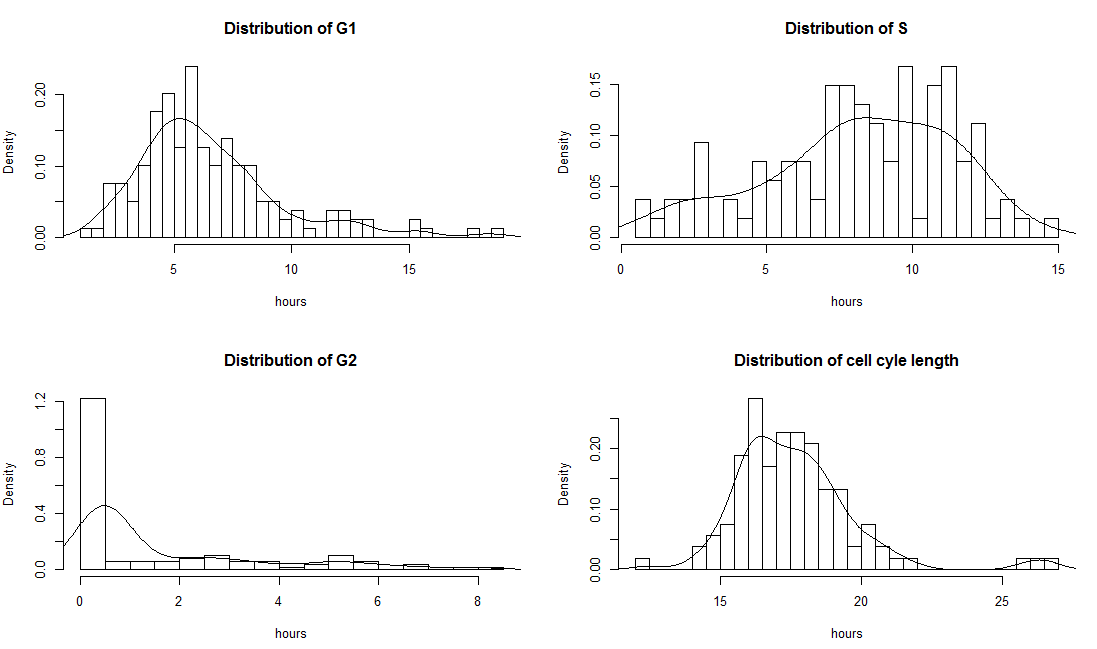
\includegraphics[width=\textwidth]{Images/Zurich.png}
\caption{Distribution of phases length on the \texttt{PCNA} data set.}
\label{fig: resPCNA}
\end{figure} 
We can also plot the distributions of each of these results, see figure \ref{fig: resPCNA}. What we first notice is that the length of phase \textit{S} is superior to the length of \textit{G1}. Out of the 234 trajectories that fulfil score 1, our classifier only predicts 106 full cycles. As expected, \textit{G2}'s length is very badly estimated, and we also notice it with the distribution estimations. However the other distributions are neat even with the counter intuitive means of lengths of the two first phases.


\subsubsection{On the MitoCheck data set without reweighting}
\begin{table}[!ht]
\centering
\begin{tabular}{|c|c|c|c|}
  \hline
  Length of:  & Mean & Standard deviation & Number of trajectories \\
  \hline
\text{G1} & 11.76 & 6.27 & 277 \\
  \hline
\text{S}  & 5.81 & 3.64 & 194 \\
  \hline
\text{G2} & 5.19 & 4.19 & 29 \\
  \hline
\text{Cell Cycle} & 23.00 & 3.94 & 29 \\
  \hline 
\end{tabular} 
  \caption{Basic characteristics of phases length on the MitoCheck data set.}
\end{table}

\begin{figure}[!ht]
\centering
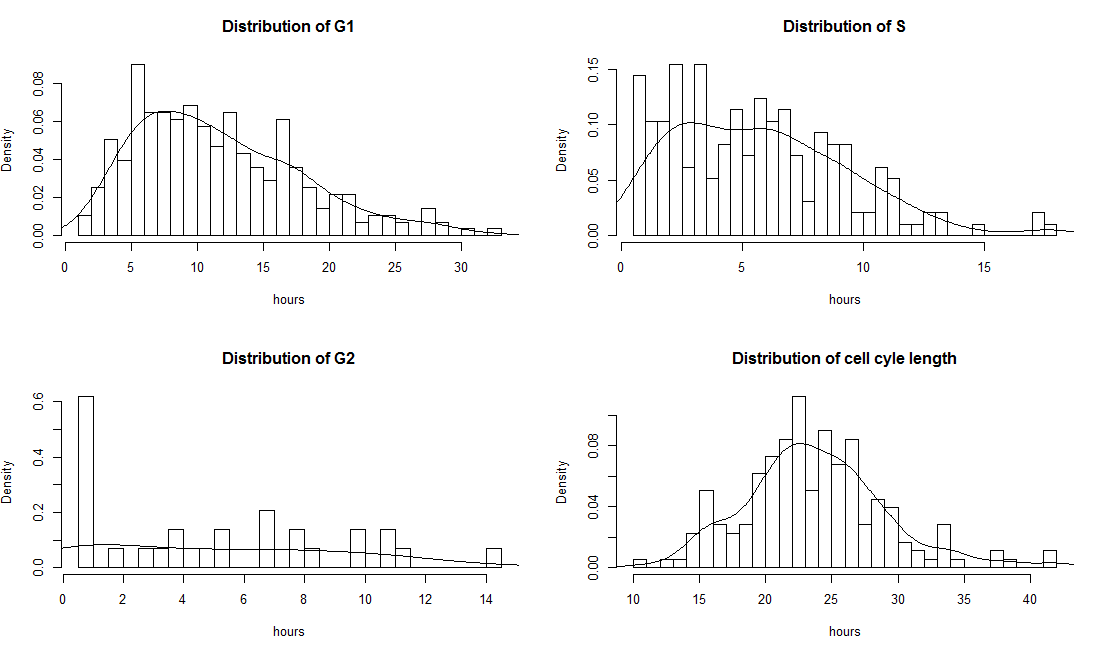
\includegraphics[width=\textwidth]{Images/MitoCheck0wieght.png}
\caption{Distribution of phases length on the MitoCheck data set.}
\label{fig: resMitoCheck}
\end{figure} 


We can also plot the distributions of each of these results, see figure \ref{fig: resMitoCheck} . Out of the 2408 trajectories that fulfil score 1, our classifier only predicts 29 full cycles. What we first notice, contrary to the \texttt{PCNA} data set, is that the length of phase \textit{G1} is superior to the length of \textit{S} and this phase length is superior to the final phase \textit{G2}. The estimation of \textit{G1}'s length is close to what we would expect, the values for the lengths of \textit{S} and \textit{G2} are not too close to literature.

\subsection{Domain Adaptation with instances reweighting}



One of the key assumptions in machine learning and data mining algorithms is that the training and future data must be in the same feature space and must have the same distribution. However, in many real world applications these assumptions are not fully validated. It seems natural that our training set was taken under some circumstances and that our test set was taken under others. It is usually not necessary to adjust the algorithms in order to take into account these differences but in some particular cases it can increase the prediction rates. Transfer learning or domain adaptation is the study of how we should adapt the learning method or the feature space in order to take into account these differences. In our case, we wish to improve the previous results by transfer learning and in particular by instance knowledge transfer. This means that we are going to alter the learning algorithm in order to learn with better suited training instances. These better suited training instances are chosen if they represent the future dataset. From a Bayesian perspective, we make the hypothesis that our training set (respectively the future data) depends on a hidden variable $\lambda$ (resp. $\theta$), let's denote by $p_{\lambda}$ (resp. $p_{\theta}$) the probability distribution of the training set (resp. of the future data). We then weight each instance $x_i$ of the training set by $\frac{p_{\theta}(x_i)}{p_{\lambda}(x_i)}$. Many other transfer learning via instances use Bayesian frameworks, in most they try to find relations between the hidden variables $\lambda$ and $\theta$. From a frequentist point of view, we make the assumption that the distribution of labels given the data is the same in both data sets. Domain adaptation can also be referred to as transfer learning with instances and by covariate shift.
\subsubsection{Method 1}

The first method is straightforward. Estimate the training distribution, estimate the future data distribution and then take the ratio of the estimated densities on each instance, see figure \ref{fig: Method1}. The denominator won't be zero because the training instance is from the training distribution, so $p_{\theta}(x_i) \neq 0$. We usually adopt kernel method density estimation. This method doesn't work in practice when the number of features is large. Some may find that even 6 dimensions is too big for kernel density estimation. Because of the curse of dimensionality, increasing the number of dimensions will decrease precision of the estimation of both distribution and will drastically increase computation time. Furthermore, because we have to take the ratio of both estimated densities, small errors in estimating $\PR$ can lead to a large coefficient which will then lead to large differences. The training will be based on wrong weights and the final predictions will be poor. This method wasn't possible, even by reducing the number of variables to 6. The selection of these 6 features was done with respect to the sensitivity of each feature to the output. The computation time to estimate the distribution of the future data on these 6 features was too great. I recall that we have over 80 000 instances and 6 dimensions. A stronger analysis of this situation can be interesting as these 6 features may not be the most characteristic for the data set as they may be strongly correlated. It may be efficient to use a principal component analysis in order to reduce de number of dimensionality and to make them uncorrelated, which would work nicely for the density estimations.

\begin{figure}[!ht]
\centering
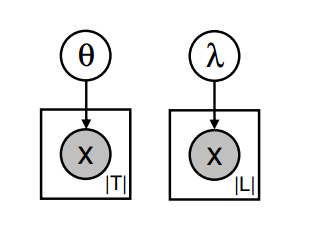
\includegraphics[width=0.3\textwidth]{Images/Method1.png}
\caption{Learning under covariate shift by estimating training
and test densities separately (image taken from \cite{pict})}
\label{fig: Method1}
\end{figure}



\subsubsection{Method 2}

A more reasonable estimation of the weight is possible by not having to estimate the full data distributions. To do so, Huang et al., see \cite{KMM} suggest turning this problem into an optimization problem. \\
Formally speaking, we have training samples $Z=\lbrace (x_1,y_1),...,(x_m,y_m) \rbrace \subseteq \mathcal{X} \times \mathcal{Y}$, where $\mathcal{X}$ is the feature space and $\mathcal{Y}$ is the space of labels. This training sample was drawn from a probability distribution $\text{Pr}(x,y)$ and the same with the future data named $Z'$ that were drawn from $\text{Pr'}(x,y)$, the labels in $Z'$ are unknown to us. The key assumption is that given the data, the distribution of labels is the same, we have $\PR(y|x)=\PR'(y|x)$. \\
The task at hand is to minimize the expected risk of the future data set with respect to a certain loss function $l:\mathcal{X}\times\mathcal{Y}:\rightarrow \mathbb{R}^+$:
$$ R[\PR',l(x,y)]=\mathbb{E}_{(x,y)\sim \PR'}[l(x,y)]$$
However, if $\PR=\PR'$ we could train on the labelled data and any machine learning algorithm would minimize this expected risk. We have the following equalities:

\begin{align*}
R[\PR',l(x,y)] &= \mathbb{E}_{(x,y)\sim\PR'}[l(x,y)] \\
               &= \mathbb{E}_{(x,y)\sim\PR}[\frac{\PR'(x,y)}{\PR(x,y)}l(x,y)] \ \text{(Same \ technics \ as \ in \ importance \ sampling)}\\ 
               &= \mathbb{E}_{(x,y)\sim\PR}[\beta(x,y)l(x,y)] \\
               &= R[\PR,\beta(x,y)l(x,y)]
\end{align*}

Where $\beta(x,y)=\frac{\PR'(x,y)}{\PR(x,y)}=\frac{\PR'(x)\PR'(y|x)}{\PR(x)\PR(y|x)}=\frac{\PR'(x)}{\PR(x)}$ is the key assumption in this setting. Like in importance sampling, we need the support of $\PR'$ to be contained in the support of $\PR$, if not we cannot make the ratio. The equality over both expected risks shows that we can minimize the expected risk of the future data by minimizing the expected risk of the training data weighted by $\beta$. \\
We will present the main theorems and optimization problem to solve this, but for more details please refer to \cite{KMM}. Let's denote by $\Phi:\mathcal{X}\rightarrow \mathcal{F}$ to be a map into a feature space $\mathcal{F}$ and denote by $\mu:\mathcal{P}\rightarrow\mathcal{F}$ the expectation operator, $\mu(\PR)=\mathbb{E}_{x\sim\PR(x)}[\phi(x)]$. As in many kernel settings we make the assumption that $\mathcal{F}$ is a reproductive kernel Hilbert space. Every function of this particular space is invariant by dot product with a kernel. We can infer a suitable $\beta$ by solving this optimization problem:
$$ \underset{\beta}{\text{minimize}} \ ||\mu(\PR')-\mathbb{E}_{x\sim \PR}[\beta(x)\phi(x)]|| \text{\ subject \ to} \ \beta(x) \geq 0 \ \text{and} \ \mathonebb{E}_{x \sim \PR(x)}[\beta(x)]=1.$$
As $\mu(\PR')$ and $\PR$ are unknown and that we only have two samples of finite size, one for training and the other for prediction we have to ensure that the empirical estimates of these quantities converge with a reasonable standard error. We have the following results on the convergences: \\
If $\beta(x)$ is bounded by $B$ and if $\beta(x)$ for $x\sim \PR$ has finite mean and non-zero variance then $\frac{1}{m}\sum_i \beta(x_i)$ converges in distribution to a gaussian distribution with mean $\int \beta(x)d\PR(x)$ and standard error $\frac{B}{2\sqrt{m}}$. \\
The convergences, like with the central limit theorem, is in $O(1/\sqrt{m})$.
The second results demonstrates the deviation between the empirical means of $\PR(x)$
and $\beta(x)\PR(x)$ in feature space given $\beta(x)$: \\
If we have $\lbrace x_1,...x_m \rbrace$ from $Z$ and $\lbrace x'_1,...x'_{m'} \rbrace$ from $Z'$ and the same conditions as before on $\beta(x)$, and if the feature map is bounded by $R$, i.e. for all $x \in \mathcal{X}$, $||\phi (x)|| \leq R$ then with probability $1-\delta$, given $\beta$, we have:
$$||\frac{1}{m}\underset{i=1}{\overset{m}{\sum}}\beta(x_i)\phi(x_i) - \frac{1}{m'}\underset{i=1}{\overset{m'}{\sum}}\phi(x'_i)|| \leq (1+\sqrt{-2\log (\delta/2)})R\sqrt{B^2/m+1/m'}  $$
This second result gives us an upper bound on the difference of the empirical means if $\beta$ is optimal, with respect towards the population. It is no guarantee that the empirical means should match and the convergence is in $O(\sqrt{1/m+1/(m'B^2)}$. \\
We wish to minimize the discrepancy between means subject to constraints $\beta_i \in [0;B]$ and $|\frac{1}{m}\sum \beta_i-1|\leq \epsilon$. Minimizing the discrepancy to minimize the gap between $\PR'$ and $\beta \PR$, whereas the second constraints ensure that $\beta \PR$ is close to a probability distribution, see the first result on the convergences. One may check that we have the following equality:
$$||\frac{1}{m}\underset{i=1}{\overset{m}{\sum}}\beta(x_i)\phi(x_i) - \frac{1}{m'}\underset{i=1}{\overset{m'}{\sum}}\phi(x'_i)|| = \frac{1}{m^2}\beta^T K \beta - \frac{2}{m^2} \kappa^T\beta + \text{const} $$ 
Where $K$ is a $m \times m$ matrix and for all $i, j$ we have $K_{ij}=k(x_i,x_j)$ and $\kappa$ is a $m$ sized vector where for all $i$, $\kappa_i=\frac{m}{m'}\underset{j=1}{\overset{m'}{\sum}}k(x_i,x'_j)$. 
The optimization problem can therefore be rewritten as: 
$$\underset{\beta}{\text{minimize}} \frac{1}{2}\beta^TK\beta-\kappa^T\beta \text{\ subject \ to } \beta_i \in [0;B] \text{\ and \ } |\underset{i=1}{\overset{m}{\sum}}\beta_i-m | \leq m\epsilon$$.



\subsubsection{Weighted Random Forest}

Both of these methods rely on a weighted classification; however in most packages and in most computing languages weighted classification algorithms are not yet implemented. Because of the simplicity of tuning of the random forest and of its efficiency we decided to only explain how we weight the instances within a random forest. We are first going to explain random forests as they were first implemented by Breiman in 2001. If we wish to construct $N\_trees$ on a data set of size $N$, we have the following algorithm:


\begin{algorithm}[!ht]
\KwResult{A regression or classification model.}
 \algorithmicrequire $\ N\_trees, \ m , \ n_{min}$ \\
  \For{ $b=1,...,N\_trees$ \ }{
  \begin{enumerate}[label=(\alph*)]
  \item Draw a boostrap sample $X^*$ of size N from the training data. 
  \item Grow a random-forest tree $T_b$ to the bootsrapped data, by recursively repating the following steps for each terminal node of the tree, until the minimum node size $n_{min}$ is reached. 
  \begin{enumerate}[label=(\roman*)]
  \item Select $m$ variables at random from the $p$ variables. 
  \item Pick the best variables/split-point among the $m$. 
  \item Split the node into two daughter nodes.
  \end{enumerate}
  \end{enumerate}
  }
 \algorithmicensure  Ensemble of trees $\lbrace T_b \rbrace_1^{N\_trees}$.
 \caption{Random Forest for Regression or Classification.}
 \label{algo:1}
\end{algorithm}

To make a prediction at a new point $x$: \\
\textit{Regression:} $\hat{f}_{\text{rf}}^{N\_tree}(x)=\frac{1}{N\_tree}\underset{b=1}{\overset{N\_tree}{\sum}}T_b(x)$\\
\textit{Classifications:} Let $\hat{C}_b(x)$ be the class prediction of the $b$-t random-forest tree. Then $\hat{C}_{\text{rf}}^{N\_tree}(x) = majority \ vote \ \lbrace \hat{C}_b(x) \rbrace_1^{N\_tree} $. \\
The weighting procedure we apply in our context is based on the training of each individual tree. Therefore we wish to give more times (with respect to its weight) samples when we train an individual tree. As they are implemented in R or Python, the classifier does a uniform bootstrap on the whole training set. Therefore, making a weighted random forest implies modifying the bootstrap procedure in order to sample with weights. However, it is not the most practical way to alter these procedures, especially in R. It would be easier with Python as we can easily access the source code within the package. In order to not alter the standard procedure we use a trick: as the bootstrap method will resample from the training set at each iteration, we will repeat the instances in the original training set according to their weight. In other words, we create a training set of size 1000 (more than twice the size of the original data set), where sample $i$ is repeated $\hat{\beta_i}\frac{1000}{\sum_j \hat{\beta_j}}$.

\subsection{Discussion about the domain adaptation technics}



\subsubsection{Tuning}

Huang et al. in figure \cite{KMM} discuss how to choose each parameter. There are 3 parameters to choose: the choice of the kernel and the associated hyper-parameters, the upper-bound $B$ of the weight coefficients and the $\epsilon$ a "closeness" parameter. Let’s comment each of these tuning parameters. \\
The kernel choice will have impacts on the kernel matrix $K$ and the vector $\kappa$. $K$ can be seen a weight matrix in the reproductive kernel Hilbert space. If we choose a 0-mean gaussian kernel which has a hyper parameter $\sigma$, the impact in variation of $\sigma$ can be seen as how many neighbours do we wish to associate with a certain instance. Choosing a small $\sigma$ will result in a stronger discrimination of each instance, or in other words creating smaller "neighbourhoods" for each instance. However if the neighbourhood is too small, everybody may have the same weights. Choosing a bigger $\sigma$ will results in bigger "neighbourhoods". We expect, if the training data and the future data feature space are close, that the choice of $\sigma$ will have little impact in the weighting scheme, whereas on the contrary, a stronger discrimination may put forward better suited instances. If no instances are better suited a smaller $\sigma$ will result in all samples having the same weight, because no samples will get "close enough". We try with $\sigma=1$ and $\sigma=10$. \\
The upper-bound $B$ on the coefficients forces values to stay reasonable, as the average of $\beta$ is close to 1, the optimization problem may want to be very discriminative by setting most coefficients to 0 and by setting only a few to high values. In Huang et al., they suggest that $B=1000$ is a suitable value. In our case, having $B=1000$ will result in a standard error on the estimation of $\beta$ of $\frac{B}{2\sqrt{m}}=\frac{1000}{2\sqrt{472}} \approx 23 $. Reducing $B$ in our case will strongly improve the validation of the second constraint, that is that $\beta\PR$ must be close to probability distribution. We try for several values of $B=2,\ 10, \ 50$ and $1000$. \\
The final tuning parameter is $\epsilon$. $\epsilon$ is involved in the second optimization constraint on the precision of the average of $\beta$ to 1. He is closely related to $B$ and will have the same impact. In Huang et al., they suggest to choose $\epsilon = \frac{\sqrt{m}-1}{\sqrt{m}}= \frac{\sqrt{472}-1}{\sqrt{472}}=\approx 0.95$. We try 3 values of $\epsilon$, $\epsilon = 0.1, \ 0.5 \ \text{and} \ 0.9$.

\subsubsection{Results}

The estimations of each phase length are exposed in table \ref{tab: resMito}. As expected the results for the lengths of phases \textit{S} ans \textit{G2} are lot poorer than for \textit{G1}. Out of the 2380 trajectories, we accept a lot more trajectories for phase \textit{G1} and \textit{S} for $\sigma=1$ then for $\sigma=10$. It is not apparent for $\sigma=1$ and we will explain why after but the number of trajectories accepted increases with the decrease of $B$ and with the decrease of $\epsilon$. This can be due to the fact that when $B$ or $\epsilon$ is large, our weight vector $\beta$ is sparse and has only a few very large weights. For some values of $B$ and $\epsilon$ the model only trains on no more than 20 different instances. In figure \ref{fig: B_decrease} and \ref{fig: eps_decrease} we see how the values of $B$ and $\epsilon$ change the weights. We would like to favour a model which will be able to train on a sufficient amount of instances. In figure \ref{fig: B_decrease}, for $B=1000, \ \epsilon=0.9$ and $\sigma=10$ we have no more than 20 instances with weights higher than 1. Let’s discuss $\sigma=1$, if we would plot the same graphs, we would be confused by the result at first. For a fixed $\epsilon$, the graphs are identical as we can see in figure \ref{fig: Sigma_one}. When $\sigma=1$, most of the weights seem to take the value of the given $\epsilon$ and the scheme down weights not well suited instances. $\epsilon = 0.1 $ yields the most variations in $\hat{\beta}$ and figure \ref{fig: Sigma_one} also shows why the results are similar for $\sigma=1$. If we try to compare the weighting for $\sigma=1$ and $\sigma=10$, we notice that the same instances are chosen or kept (for $\sigma=1$ these are the "flat regions" whereas for $\sigma=10$, this corresponds to the "spiky areas"). \\
To conclude we would choose the weighting scheme that keeps the most instances while selecting still selecting those that are better suited. In this case, $\sigma=10$ chooses too few instances. For $\sigma=1$ the choice of $B$ does not matter much, so we would choose $\epsilon=0.9$ to increase the variation in the weighting scheme. We would choose, $\sigma=1, \ B=10$ and $\epsilon=0.9$ as parameters for our transfer learning.
\\ To be clear on the choice of $\epsilon$, if $\sigma=1$ we start with everyone, so we wish to increase variability in order to have a better selection, to increase variability we increase $\epsilon$. If $\sigma=10$, we start with nearly no one, so we wish to decrease $\epsilon$ to decrease the weights of the selected few and to increase the weights of those not selected.


\begin{table}[!ht]
\begin{tabular}{|c|c|c|c|c|c|c|c|c|c|c|c|c|c|c|}
  \hline
    \multicolumn{3}{|c|}{Paramètre} & \multicolumn{3}{|c|}{G1} & \multicolumn{3}{|c|}{S} & \multicolumn{3}{|c|}{G2} & \multicolumn{3}{|c|}{CellCycle} \\
    \hline 
    $\sigma$ &  B & $\epsilon$  & Mean & Sd  & n & Mean & Sd & n & Mean & Sd & n & Mean & Sd & n  \\
  \hline
   \color{Red} $\sigma = 1$ & 2 & 0.1 & 11.9 & 6.1 & 322 & 5.0 & 3.6 & 237 & 5.8 & 5.2 & 107 & 23.2 &3.7 & 79\\
                &   & 0.5 & 11.9 & 6.1 & 329 & 5.2 & 3.7 & 241 & 5.6 & 5.1 & 106 &22.8 &3.9 &76\\
                &   & 0.9 & 12.2 & 6.1 & 297 & 4.9 & 3.5 & 236 & 5.4 & 5.2 & 104 &22.9 &3.8 &74\\
                & \color{Red} 10 & 0.1 & 11.8  & 6.3 & 302 & 5.1 & 3.4 & 234 & 5.8 & 5.0 & 99 & 23.1& 3.9 & 72\\
                &   & 0.5 & 12.2 & 6.4 & 327 & 5.8 & 3.8 & 234 & 5.0 & 5.0 & 103 & 22.8 &3.9 &75\\
                &   & \color{Red} 0.9 & \color{Red}12 & \color{Red}6.5 & \color{Red}343 &\color{Red} 5.8 &\color{Red} 3.9 &\color{Red} 252 &\color{Red} 5.4 &\color{Red} 5.1 &\color{Red} 108 &\color{Red} 23 &\color{Red} 3.8 &\color{Red} 78\\
                & 50 & 0.1 & 12.1 & 6.1 & 274 & 4.2 & 3.2 & 239 & 6.1 & 5.1 & 104 &22.9 &3.8 &69\\
                &   & 0.5 & 11.9 & 6.3 & 313 & 5.6 & 3.8 & 233 & 5.6 & 5.1 & 102 &23.0 &3.9 &73\\
                &   & 0.9 & 11.6 & 6.1 & 333 & 5.8 & 3.7 & 238 & 5.2 & 5.0 & 107 &23.0 &3.8 &77\\
                & 1000 & 0.1 & 12.3 & 6.2 & 292 & 4.7 & 3.3 & 226 & 5.6 & 5.2 & 100 &23.0 &3.9 &71\\
                &   & 0.5 & 12.7 & 6.4 & 299 & 4.2 & 3.5 & 239 & 6.2 & 5.2 & 101 &23.0 &3.8 &73\\
                &   & 0.9 & 12.0 & 6.5 & 335 & 5.9 & 3.6 & 241 & 5.0 & 4.9 & 112 &23.1 &3.8 &80\\
\hline
  $\sigma = 10$ & 2 & 0.1 &  11.5 & 6.4 & 260 & 2.7& 2.8& 200 & 8.0 & 5.6 & 138 & 22.9 &3.8 & 92\\
                &   & 0.5 & 10.6 & 6.4 & 245 & 2.3 & 2.8 & 120 & 8.7 & 6.1 & 139 &22.9 & 3.9&84\\
                &   & 0.9 & 10.5 & 6.6 & 221 & 3.5 & 4.1 & 163 & 8.6 & 5.9 & 119 &22.9 &4 &70\\
                & 10 & 0.1 & 10.8 & 5.9 & 171 & 1.8 & 2.8 & 112 & 6.9 & 5.7 & 122 & 22.6& 3.8&60\\
                &   & 0.5 & 10.4 & 6.0 & 202 & 1.6 & 2.4 & 127 & 8.2 & 5.9 & 130 & 22.6&3.8 &60\\
                &   & 0.9 & 10.7 & 6.4 & 96 & 1.0 & 0.7 & 67 & 5.6 & 5.3 & 91 & 21.9&4.2 &36\\
                & 50 & 0.1 & 11.2 & 6.3 & 165 & 2.5 & 3.5 & 127 & 6.6 & 5.7 & 108 &22.4 &3.9 &63\\
                &   & 0.5 & 15.1 & 8.8 & 52 & 1.2 & 0.8 & 61 & 2.9 & 4.0 & 74 &21.7 & 3.9&63\\
                &   & 0.9 & 14.5 & 8.4 & 55 & 1.2 & 0.8 & 53 & 2.1 & 2.7 & 81 &20.1 &4.9 &15\\
                & 1000 & 0.1 & 11.6 & 6.1 & 191 & 2.7 & 3.5 & 162 & 6.5 & 5.6 & 107 &22.5 &3.8 &65\\
                &   & 0.5 & 13.8 & 7.6 & 64 & 1.1 & 0.6 & 40 & 3.5 & 4.2 & 66 &20.4 &4.7 &18\\
                &   & 0.9 & 12.2 & 6.9 & 89 & 1.4 & 0.9 & 74 & 3.9 & 4.5 & 95 &21.1 &4.8 &23\\
  \hline
\end{tabular}
\caption{Different estimations of phase length on the MitoCheck dataset.}
\label{tab: resMito}
\end{table}


\begin{figure}
\centering
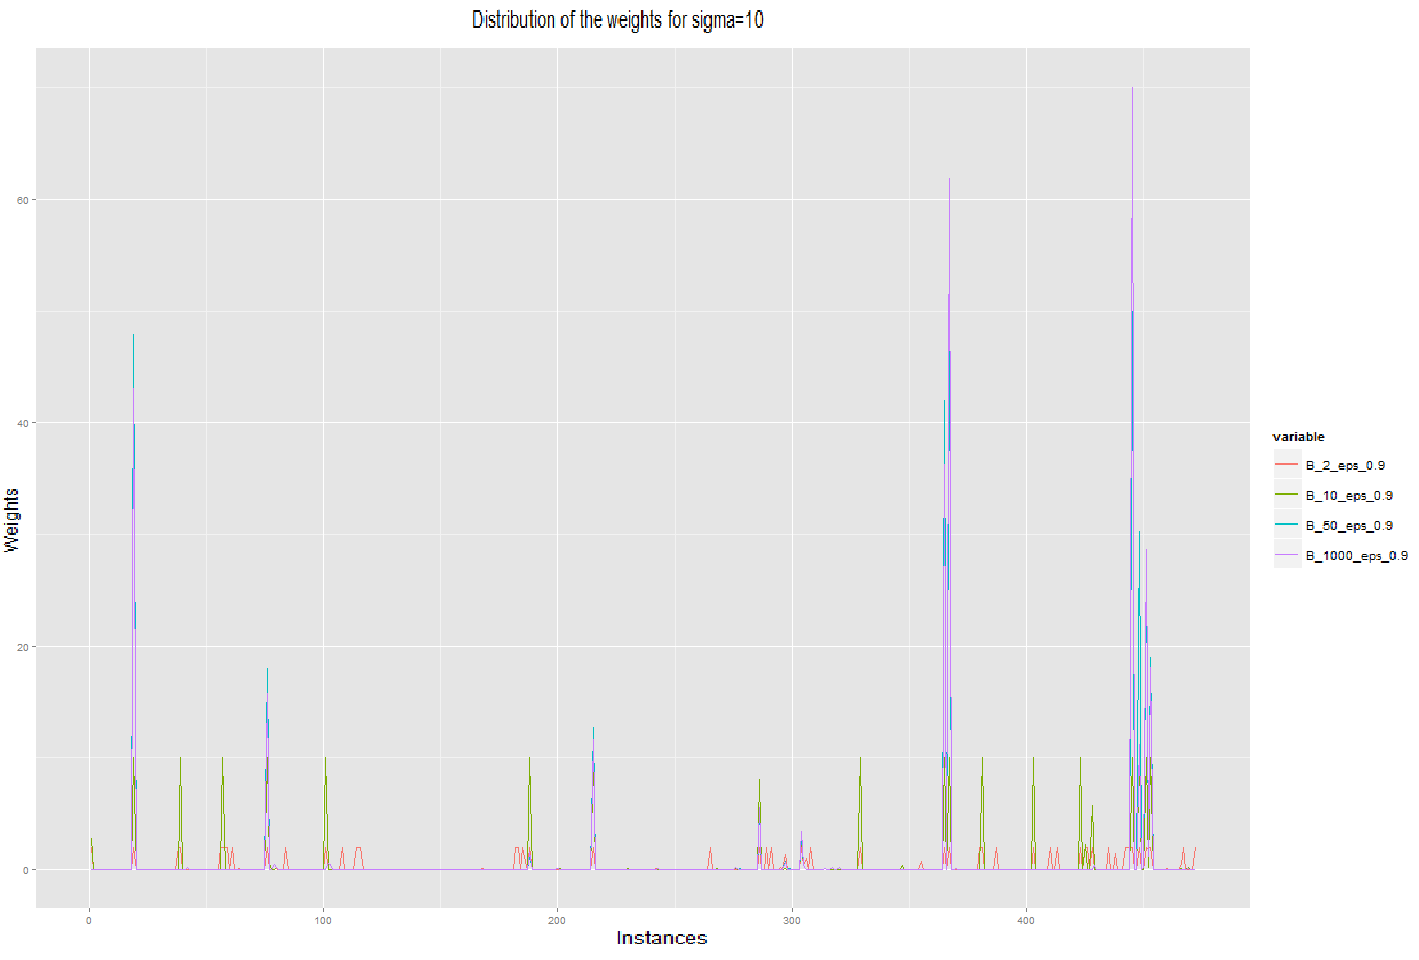
\includegraphics[width=\textwidth,height=7cm]{Images/Weights_B_10.png}
\caption{How the weighting scheme varies when $B$ decreases ($\sigma=10$).}
\label{fig: B_decrease}
\end{figure}

\begin{figure}
\centering
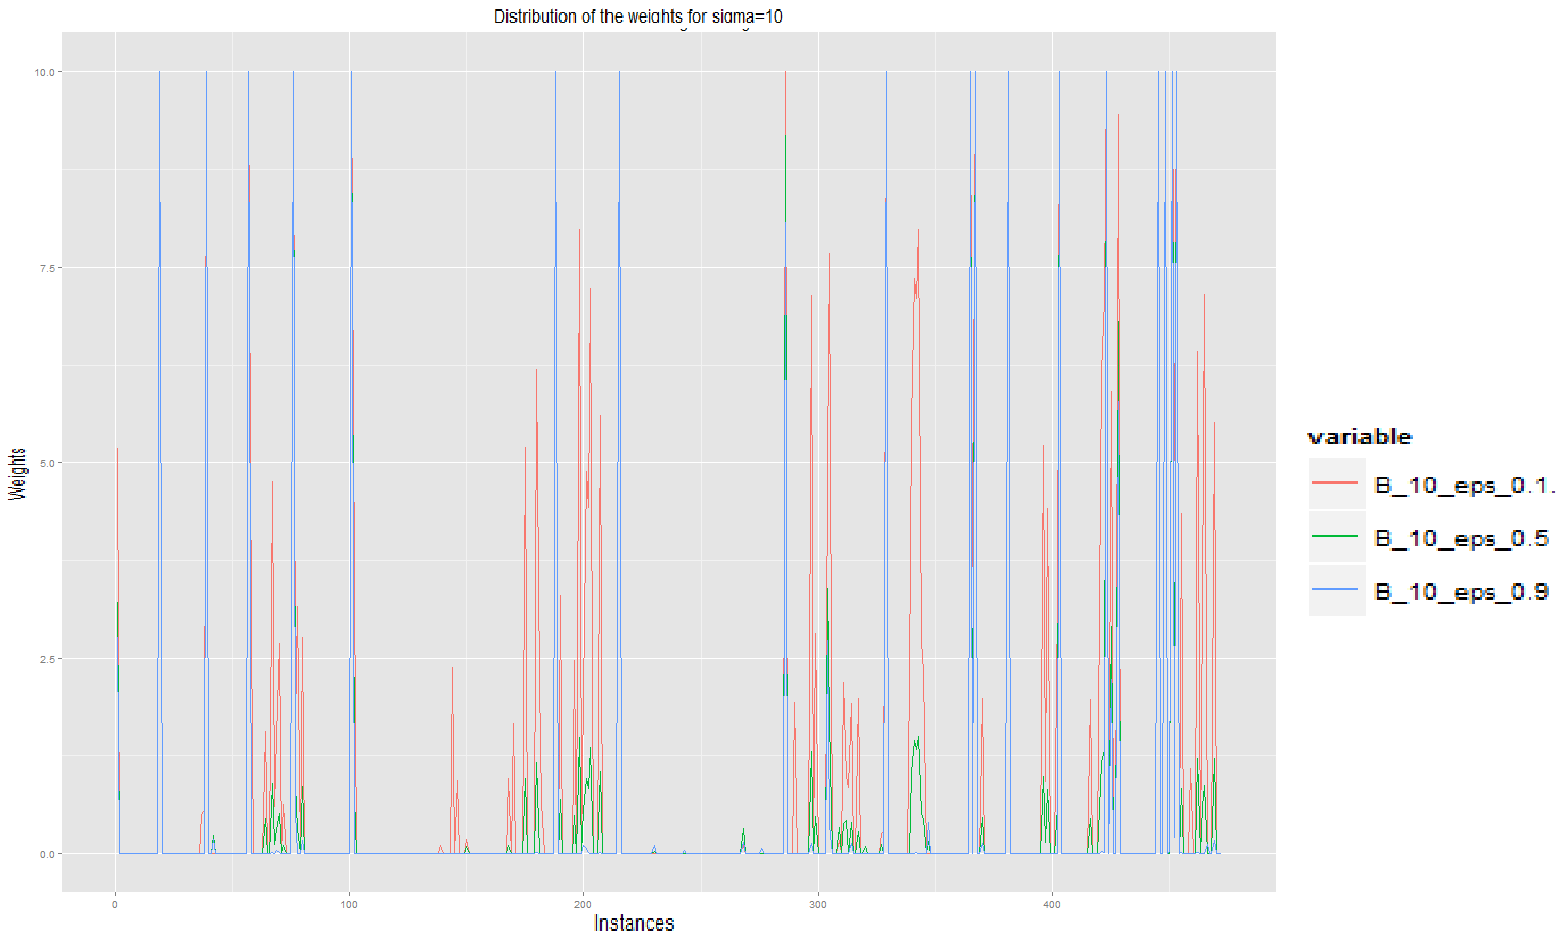
\includegraphics[width=\textwidth,height=7cm]{Images/Weights_eps_10.png}
\caption{How the weighting scheme varies when $\epsilon$ decreases ($\sigma=10$).}
\label{fig: eps_decrease}
\end{figure}

\begin{figure}
\centering
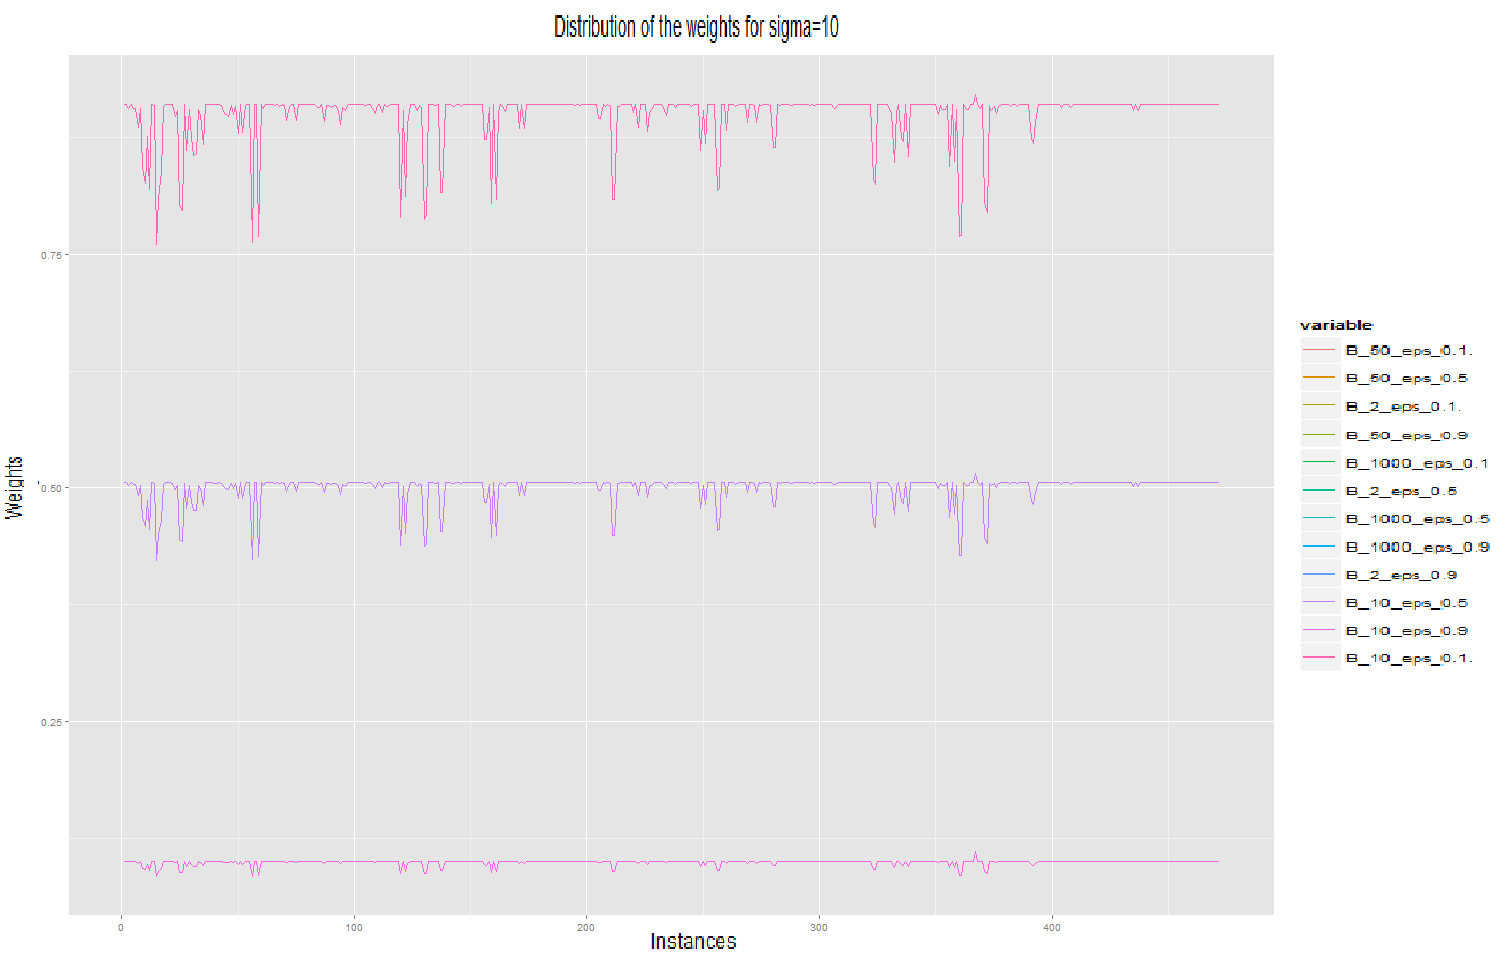
\includegraphics[width=\textwidth,height=8cm]{Images/Sigma_one.png}
\caption{How the weighting scheme varies when $\epsilon$ and $B$ vary ($\sigma=1$).}
\label{fig: Sigma_one}
\end{figure}

\clearpage

\section{Conclusion}

I studied whether or not it was possible to detect the non-mitotic cell cycle phases with the \texttt{H2B} marker alone. This fluorescent marker is informative about mitotic events, so it is not guaranteed that we could detect the different non-mitotic phases with the \texttt{H2B} marker alone. On the contrary to the \texttt{PCNA} marker, which is informative about the non-mitotic phases \textit{G1}, \textit{S} and \textit{G2}. The \texttt{PCNA} marker enables us to use a labelled MitoCheck-like data set for training. This training allowed us to infer predictive models for the lengths of the different phases \textit{G1}, \textit{S} and \textit{G2}. But with no ground truth on the future data set it may seem difficult to assess how good our classifiers perform.

\bigskip

The data set is composed of trajectories from different wells. The data was transformed only for the second classifier. A normalization process strongly improved the prediction rate as it takes into account time dependencies and cell evolution through time. Our final classifier combines 2 classification models and a correcting model. The first classifier is binary and checks for mitotic or not events. The first classifier will take priority over the 3 phase random forest classifier, which is the second classifier. The error correcting model is set with a strong prior based on biology beliefs and takes time dependencies more strongly into account. We achieve 86\% accuracy on the labelled training set. We can only efficiently detect the transition between phase \textit{G1} and \textit{S}. It can seem fairly natural as even with our own eye it is hard to distinguish the two events. 

\bigskip

The classifier was then used on data from a published genome-wide screen, generated by the FP6-financed European Union project, MitoCheck. The MitoCheck data set is a collection of loss-of-function protein experiments where the \texttt{H2B} marker is the only used fluorescent marker. Our classifier was built with this in mind. The raw data of the MitoCheck project is different to the \texttt{PCNA} data set as we have more difficulties in estimating each phase, our classifier validates very few trajectories. This is our only criteria in addition to biological literature. To increase its performance, we use transfer instance learning on the second classifier. These methods are used when there are differences in the training and the prediction set. The one used is based on altering the training set in order to take only the best suited instances. However it is a hard task to validate the performance of our classifiers on the MitoCheck dataset without ground truth.

\bigskip

The next step of this work is to compare it with actual ground truth on the MitoCheck data set which will become available thanks to EMBL, Heidelberg. It would be nice to take time to check the distributions of the most paramount features for classification on both data set (the \texttt{PCNA} data set and the MitoCheck data set) and check that they follow similar distribution. This would allow to assess if transfer learning via instance selection is better suited than transfer learning via feature transformation. 

<We may want to relax our classifier, with the hidden Markov model perhaps, in order to track cells which may have become cancerous and therefore do not have standard behaviour.> 

If the classifier is good enough, this would enable protein function inference through loss-of-function experiments that is the MitoCheck project.

\clearpage

\section{Annexe: Hidden Markov Model}
\subsection{Emission Matrix:}

\[
  \mathbf{Emission Matrix} = 
    \begin{blockarray}{ccccc}
        & G1 & S & G2 & M\\
      \begin{block}{c(cccc)}
        G1 & .824 & .156 & .005 & .015\\
        S  & .106 & .871 & .023 & .   \\
        G2 & .    & .500 & .470 & .030\\
        M  & .033 & .033 & .033 & .901\\
      \end{block}
    \end{blockarray}
\]

$0.023$ is equal to the probability of being in the actual state "S" but the classifier says that he is "G2".

\subsection{Transition Matrix for the \texttt{PCNA} data set:}
\[
  \mathbf{Transition Matrix PCNA} = 
    \begin{blockarray}{ccccc}
        & G1 & S & G2 & M\\
      \begin{block}{c(cccc)}
        G1 & .982 & .018 & .    & .  \\
        S  & .    & .921 & .079 & .  \\
        G2 & .    & .    & .972 & .028\\
        M  & .275 & .    & .    & .725\\
      \end{block}
    \end{blockarray}
\]
$0.079$ is the probability of transiting from state "S" to state "G2".

\subsection{Transition Matrix for the \texttt{MitoCheck} data set:}

\[
  \mathbf{Transition Matrix MitoCheck} = 
    \begin{blockarray}{ccccc}
        & G1 & S & G2 & M\\
      \begin{block}{c(cccc)}
        G1 & .938 & .062 & .    & .   \\
        S  & .    & .796 & .204 & .   \\
        G2 & .    & .    & .929 & .071\\
        M  & .700 & .    & .    & .300\\
      \end{block}
    \end{blockarray}
\]

$0.204$ is the probability of transiting from state "S" to state "G2".

\subsection{Starting probability}
\[
  \mathbf{Starting Probabilities} = 
    \begin{blockarray}{cc}
      \begin{block}{c(c)}
        G1 & .72   \\
        S  & .   \\
        G2 & .   \\
        M  & .28   \\
      \end{block}
    \end{blockarray}
\]



\section{Annexe: Image}
\begin{figure}[!ht]
\centering
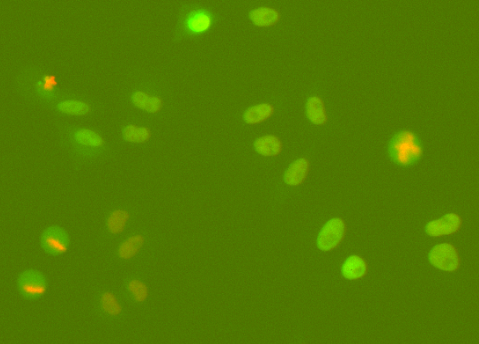
\includegraphics[width=.7\textwidth]{Images/H2B_PCNA.png}
\caption{Raw image with emission from \texttt{H2B}-mcherry (red) and from \texttt{PCNA}-EGFP (green)}
\label{fig: annexe: H2B and PCNA}
\textit{Data acquired by Michael Olma (Peter group, ETH Zurich) at a Molecular Devices ImageXpress Micro with the PlateScanPackage. They used widefield epifluorescence microscopy, 10$\times$ dry objective (0.645 $\mu$m / pixel), 1392$\times$1040 pixel, 482 frames $\times$ 5.9 min = 47.4 hours. }\\
\textit{plate \textit{LT0001\_01}, well position 0015, frame number 60}
\end{figure}

\begin{figure}[!ht]
\centering
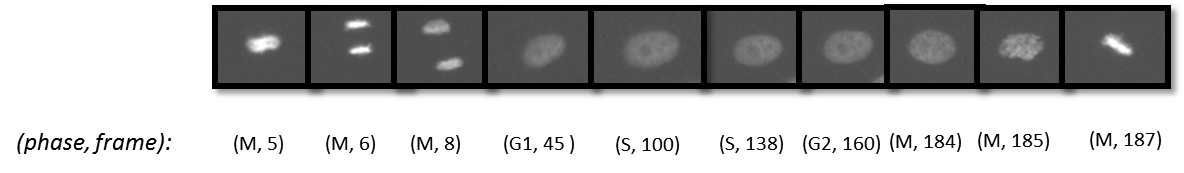
\includegraphics[width=\textwidth]{Images/traj_0_H2B.png}
\caption{Raw data for trajectory 0.}
\label{fig: annexe: RawData_traj0}
\textit{Data acquired by Michael Olma (Peter group, ETH Zurich) at a Molecular Devices ImageXpress Micro with the PlateScanPackage. They used widefield epifluorescence microscopy, 10$\times$ dry objective (0.645 $\mu$m / pixel), 1392$\times$1040 pixel, 482 frames $\times$ 5.9 min = 47.4 hours. }\\
\textit{plate \textit{LT0001\_01}, well position 0015, frame number 60}
\end{figure}

\begin{figure}[!ht]
\centering
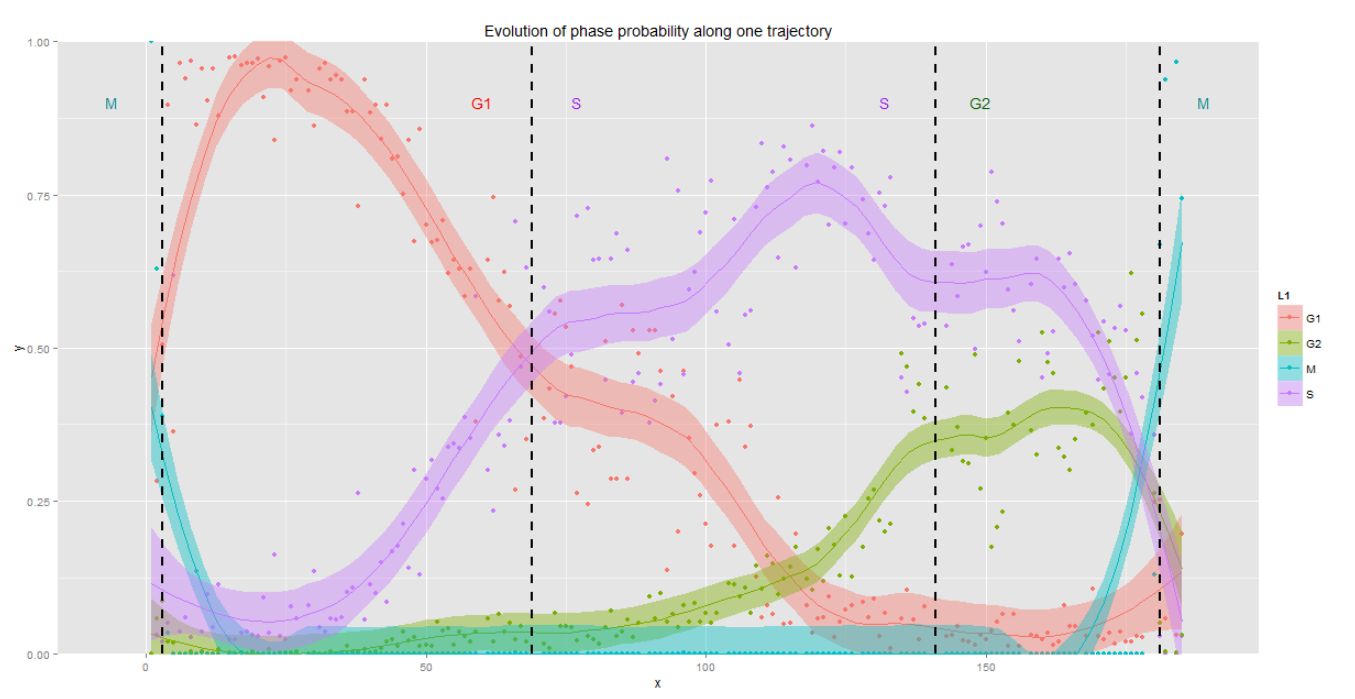
\includegraphics[width=\textwidth,height=7cm]{Images/ProbTraj_n.png}
\caption{Class probability evolution given by random forest with all four responses and the data is normalized}
\label{fig: annexe: ProbabilityEvolution_n}
\end{figure}

\begin{figure}[!ht]
\centering
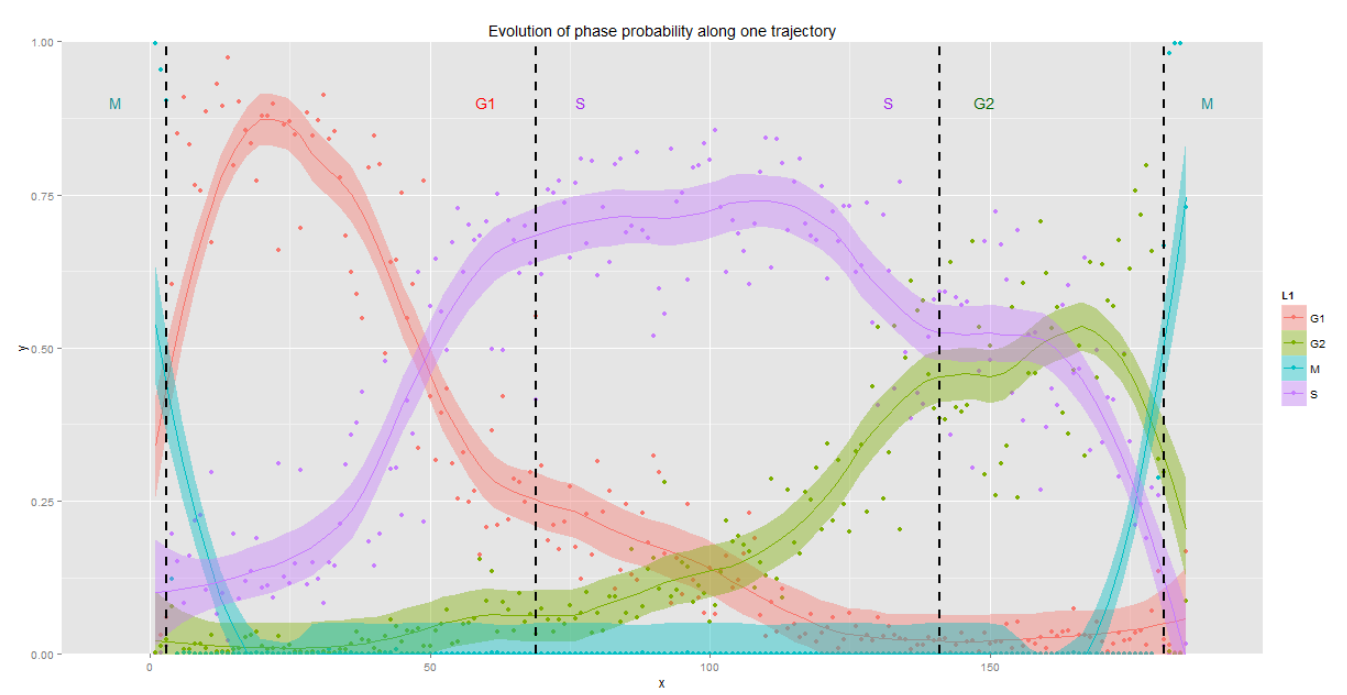
\includegraphics[width=\textwidth,height=7cm]{Images/ProbTraj_u.png}
\caption{Class probability evolution given by random forest with all four responses and the data is unnormalized}
\label{fig: annexe: ProbabilityEvolution_u}
\end{figure}

\clearpage

\begin{thebibliography}{9}

\bibitem{ThomasNature} Held M., Schmitz M.H., Fischer B., Walter T., Neumann B., Olma M.H., Peter M., Ellenberg J. \& 
Gerlich, D.W.: \textit{CellCognition: time resolved phenotype annotation in high throughput live cell imaging.} \textbf{Nature Methods.} August 2010.


\bibitem{MitoCheck} Presentation of the MitoCheck project, \texttt{http://www.mitocheck.org/}.


\bibitem{CellCognition} The CellCognition software and presentation, \texttt{http://www.cellcognition.org/}.


\bibitem{Features} \textit{Technical Report: Feature extraction}, Walter T. January 2007. The paper was added to the annexe, in the following pages.

\bibitem{KMM} Huang, Jiayuan, et al. \textit{Correcting sample selection bias by unlabeled data.} Advances in neural information processing systems. 2006.

\bibitem{pict} Bickel, Steffen, Michael Brückner, and Tobias Scheffer. "Discriminative learning for differing training and test distributions." Proceedings of the 24th international conference on Machine learning. ACM, 2007.
\end{thebibliography}


\includepdf[pages={1,2,3,4,5,6,7,8,9,10,11}]{features.pdf}

\end{document}

